
    




    
\documentclass[11pt]{article}

    
    \usepackage[breakable]{tcolorbox}
    \tcbset{nobeforeafter} % prevents tcolorboxes being placing in paragraphs
    \usepackage{float}
    \floatplacement{figure}{H} % forces figures to be placed at the correct location
    
    \usepackage[T1]{fontenc}
    % Nicer default font (+ math font) than Computer Modern for most use cases
    \usepackage{mathpazo}

    % Basic figure setup, for now with no caption control since it's done
    % automatically by Pandoc (which extracts ![](path) syntax from Markdown).
    \usepackage{graphicx}
    % We will generate all images so they have a width \maxwidth. This means
    % that they will get their normal width if they fit onto the page, but
    % are scaled down if they would overflow the margins.
    \makeatletter
    \def\maxwidth{\ifdim\Gin@nat@width>\linewidth\linewidth
    \else\Gin@nat@width\fi}
    \makeatother
    \let\Oldincludegraphics\includegraphics
    % Set max figure width to be 80% of text width, for now hardcoded.
    \renewcommand{\includegraphics}[1]{\Oldincludegraphics[width=.8\maxwidth]{#1}}
    % Ensure that by default, figures have no caption (until we provide a
    % proper Figure object with a Caption API and a way to capture that
    % in the conversion process - todo).
    \usepackage{caption}
    \DeclareCaptionLabelFormat{nolabel}{}
    \captionsetup{labelformat=nolabel}

    \usepackage{adjustbox} % Used to constrain images to a maximum size 
    \usepackage{xcolor} % Allow colors to be defined
    \usepackage{enumerate} % Needed for markdown enumerations to work
    \usepackage{geometry} % Used to adjust the document margins
    \usepackage{amsmath} % Equations
    \usepackage{amssymb} % Equations
    \usepackage{textcomp} % defines textquotesingle
    % Hack from http://tex.stackexchange.com/a/47451/13684:
    \AtBeginDocument{%
        \def\PYZsq{\textquotesingle}% Upright quotes in Pygmentized code
    }
    \usepackage{upquote} % Upright quotes for verbatim code
    \usepackage{eurosym} % defines \euro
    \usepackage[mathletters]{ucs} % Extended unicode (utf-8) support
    \usepackage[utf8x]{inputenc} % Allow utf-8 characters in the tex document
    \usepackage{fancyvrb} % verbatim replacement that allows latex
    \usepackage{grffile} % extends the file name processing of package graphics 
                         % to support a larger range 
    % The hyperref package gives us a pdf with properly built
    % internal navigation ('pdf bookmarks' for the table of contents,
    % internal cross-reference links, web links for URLs, etc.)
    \usepackage{hyperref}
    \usepackage{longtable} % longtable support required by pandoc >1.10
    \usepackage{booktabs}  % table support for pandoc > 1.12.2
    \usepackage[inline]{enumitem} % IRkernel/repr support (it uses the enumerate* environment)
    \usepackage[normalem]{ulem} % ulem is needed to support strikethroughs (\sout)
                                % normalem makes italics be italics, not underlines
    \usepackage{mathrsfs}
    

    
    % Colors for the hyperref package
    \definecolor{urlcolor}{rgb}{0,.145,.698}
    \definecolor{linkcolor}{rgb}{.71,0.21,0.01}
    \definecolor{citecolor}{rgb}{.12,.54,.11}

    % ANSI colors
    \definecolor{ansi-black}{HTML}{3E424D}
    \definecolor{ansi-black-intense}{HTML}{282C36}
    \definecolor{ansi-red}{HTML}{E75C58}
    \definecolor{ansi-red-intense}{HTML}{B22B31}
    \definecolor{ansi-green}{HTML}{00A250}
    \definecolor{ansi-green-intense}{HTML}{007427}
    \definecolor{ansi-yellow}{HTML}{DDB62B}
    \definecolor{ansi-yellow-intense}{HTML}{B27D12}
    \definecolor{ansi-blue}{HTML}{208FFB}
    \definecolor{ansi-blue-intense}{HTML}{0065CA}
    \definecolor{ansi-magenta}{HTML}{D160C4}
    \definecolor{ansi-magenta-intense}{HTML}{A03196}
    \definecolor{ansi-cyan}{HTML}{60C6C8}
    \definecolor{ansi-cyan-intense}{HTML}{258F8F}
    \definecolor{ansi-white}{HTML}{C5C1B4}
    \definecolor{ansi-white-intense}{HTML}{A1A6B2}
    \definecolor{ansi-default-inverse-fg}{HTML}{FFFFFF}
    \definecolor{ansi-default-inverse-bg}{HTML}{000000}

    % commands and environments needed by pandoc snippets
    % extracted from the output of `pandoc -s`
    \providecommand{\tightlist}{%
      \setlength{\itemsep}{0pt}\setlength{\parskip}{0pt}}
    \DefineVerbatimEnvironment{Highlighting}{Verbatim}{commandchars=\\\{\}}
    % Add ',fontsize=\small' for more characters per line
    \newenvironment{Shaded}{}{}
    \newcommand{\KeywordTok}[1]{\textcolor[rgb]{0.00,0.44,0.13}{\textbf{{#1}}}}
    \newcommand{\DataTypeTok}[1]{\textcolor[rgb]{0.56,0.13,0.00}{{#1}}}
    \newcommand{\DecValTok}[1]{\textcolor[rgb]{0.25,0.63,0.44}{{#1}}}
    \newcommand{\BaseNTok}[1]{\textcolor[rgb]{0.25,0.63,0.44}{{#1}}}
    \newcommand{\FloatTok}[1]{\textcolor[rgb]{0.25,0.63,0.44}{{#1}}}
    \newcommand{\CharTok}[1]{\textcolor[rgb]{0.25,0.44,0.63}{{#1}}}
    \newcommand{\StringTok}[1]{\textcolor[rgb]{0.25,0.44,0.63}{{#1}}}
    \newcommand{\CommentTok}[1]{\textcolor[rgb]{0.38,0.63,0.69}{\textit{{#1}}}}
    \newcommand{\OtherTok}[1]{\textcolor[rgb]{0.00,0.44,0.13}{{#1}}}
    \newcommand{\AlertTok}[1]{\textcolor[rgb]{1.00,0.00,0.00}{\textbf{{#1}}}}
    \newcommand{\FunctionTok}[1]{\textcolor[rgb]{0.02,0.16,0.49}{{#1}}}
    \newcommand{\RegionMarkerTok}[1]{{#1}}
    \newcommand{\ErrorTok}[1]{\textcolor[rgb]{1.00,0.00,0.00}{\textbf{{#1}}}}
    \newcommand{\NormalTok}[1]{{#1}}
    
    % Additional commands for more recent versions of Pandoc
    \newcommand{\ConstantTok}[1]{\textcolor[rgb]{0.53,0.00,0.00}{{#1}}}
    \newcommand{\SpecialCharTok}[1]{\textcolor[rgb]{0.25,0.44,0.63}{{#1}}}
    \newcommand{\VerbatimStringTok}[1]{\textcolor[rgb]{0.25,0.44,0.63}{{#1}}}
    \newcommand{\SpecialStringTok}[1]{\textcolor[rgb]{0.73,0.40,0.53}{{#1}}}
    \newcommand{\ImportTok}[1]{{#1}}
    \newcommand{\DocumentationTok}[1]{\textcolor[rgb]{0.73,0.13,0.13}{\textit{{#1}}}}
    \newcommand{\AnnotationTok}[1]{\textcolor[rgb]{0.38,0.63,0.69}{\textbf{\textit{{#1}}}}}
    \newcommand{\CommentVarTok}[1]{\textcolor[rgb]{0.38,0.63,0.69}{\textbf{\textit{{#1}}}}}
    \newcommand{\VariableTok}[1]{\textcolor[rgb]{0.10,0.09,0.49}{{#1}}}
    \newcommand{\ControlFlowTok}[1]{\textcolor[rgb]{0.00,0.44,0.13}{\textbf{{#1}}}}
    \newcommand{\OperatorTok}[1]{\textcolor[rgb]{0.40,0.40,0.40}{{#1}}}
    \newcommand{\BuiltInTok}[1]{{#1}}
    \newcommand{\ExtensionTok}[1]{{#1}}
    \newcommand{\PreprocessorTok}[1]{\textcolor[rgb]{0.74,0.48,0.00}{{#1}}}
    \newcommand{\AttributeTok}[1]{\textcolor[rgb]{0.49,0.56,0.16}{{#1}}}
    \newcommand{\InformationTok}[1]{\textcolor[rgb]{0.38,0.63,0.69}{\textbf{\textit{{#1}}}}}
    \newcommand{\WarningTok}[1]{\textcolor[rgb]{0.38,0.63,0.69}{\textbf{\textit{{#1}}}}}
    
    
    % Define a nice break command that doesn't care if a line doesn't already
    % exist.
    \def\br{\hspace*{\fill} \\* }
    % Math Jax compatibility definitions
    \def\gt{>}
    \def\lt{<}
    \let\Oldtex\TeX
    \let\Oldlatex\LaTeX
    \renewcommand{\TeX}{\textrm{\Oldtex}}
    \renewcommand{\LaTeX}{\textrm{\Oldlatex}}
    % Document parameters
    % Document title
    \title{cryptopals}
    
    
    
    
    
% Pygments definitions
\makeatletter
\def\PY@reset{\let\PY@it=\relax \let\PY@bf=\relax%
    \let\PY@ul=\relax \let\PY@tc=\relax%
    \let\PY@bc=\relax \let\PY@ff=\relax}
\def\PY@tok#1{\csname PY@tok@#1\endcsname}
\def\PY@toks#1+{\ifx\relax#1\empty\else%
    \PY@tok{#1}\expandafter\PY@toks\fi}
\def\PY@do#1{\PY@bc{\PY@tc{\PY@ul{%
    \PY@it{\PY@bf{\PY@ff{#1}}}}}}}
\def\PY#1#2{\PY@reset\PY@toks#1+\relax+\PY@do{#2}}

\expandafter\def\csname PY@tok@gd\endcsname{\def\PY@tc##1{\textcolor[rgb]{0.63,0.00,0.00}{##1}}}
\expandafter\def\csname PY@tok@gu\endcsname{\let\PY@bf=\textbf\def\PY@tc##1{\textcolor[rgb]{0.50,0.00,0.50}{##1}}}
\expandafter\def\csname PY@tok@gt\endcsname{\def\PY@tc##1{\textcolor[rgb]{0.00,0.27,0.87}{##1}}}
\expandafter\def\csname PY@tok@gs\endcsname{\let\PY@bf=\textbf}
\expandafter\def\csname PY@tok@gr\endcsname{\def\PY@tc##1{\textcolor[rgb]{1.00,0.00,0.00}{##1}}}
\expandafter\def\csname PY@tok@cm\endcsname{\let\PY@it=\textit\def\PY@tc##1{\textcolor[rgb]{0.25,0.50,0.50}{##1}}}
\expandafter\def\csname PY@tok@vg\endcsname{\def\PY@tc##1{\textcolor[rgb]{0.10,0.09,0.49}{##1}}}
\expandafter\def\csname PY@tok@vi\endcsname{\def\PY@tc##1{\textcolor[rgb]{0.10,0.09,0.49}{##1}}}
\expandafter\def\csname PY@tok@mh\endcsname{\def\PY@tc##1{\textcolor[rgb]{0.40,0.40,0.40}{##1}}}
\expandafter\def\csname PY@tok@cs\endcsname{\let\PY@it=\textit\def\PY@tc##1{\textcolor[rgb]{0.25,0.50,0.50}{##1}}}
\expandafter\def\csname PY@tok@ge\endcsname{\let\PY@it=\textit}
\expandafter\def\csname PY@tok@vc\endcsname{\def\PY@tc##1{\textcolor[rgb]{0.10,0.09,0.49}{##1}}}
\expandafter\def\csname PY@tok@il\endcsname{\def\PY@tc##1{\textcolor[rgb]{0.40,0.40,0.40}{##1}}}
\expandafter\def\csname PY@tok@go\endcsname{\def\PY@tc##1{\textcolor[rgb]{0.53,0.53,0.53}{##1}}}
\expandafter\def\csname PY@tok@cp\endcsname{\def\PY@tc##1{\textcolor[rgb]{0.74,0.48,0.00}{##1}}}
\expandafter\def\csname PY@tok@gi\endcsname{\def\PY@tc##1{\textcolor[rgb]{0.00,0.63,0.00}{##1}}}
\expandafter\def\csname PY@tok@gh\endcsname{\let\PY@bf=\textbf\def\PY@tc##1{\textcolor[rgb]{0.00,0.00,0.50}{##1}}}
\expandafter\def\csname PY@tok@ni\endcsname{\let\PY@bf=\textbf\def\PY@tc##1{\textcolor[rgb]{0.60,0.60,0.60}{##1}}}
\expandafter\def\csname PY@tok@nl\endcsname{\def\PY@tc##1{\textcolor[rgb]{0.63,0.63,0.00}{##1}}}
\expandafter\def\csname PY@tok@nn\endcsname{\let\PY@bf=\textbf\def\PY@tc##1{\textcolor[rgb]{0.00,0.00,1.00}{##1}}}
\expandafter\def\csname PY@tok@no\endcsname{\def\PY@tc##1{\textcolor[rgb]{0.53,0.00,0.00}{##1}}}
\expandafter\def\csname PY@tok@na\endcsname{\def\PY@tc##1{\textcolor[rgb]{0.49,0.56,0.16}{##1}}}
\expandafter\def\csname PY@tok@nb\endcsname{\def\PY@tc##1{\textcolor[rgb]{0.00,0.50,0.00}{##1}}}
\expandafter\def\csname PY@tok@nc\endcsname{\let\PY@bf=\textbf\def\PY@tc##1{\textcolor[rgb]{0.00,0.00,1.00}{##1}}}
\expandafter\def\csname PY@tok@nd\endcsname{\def\PY@tc##1{\textcolor[rgb]{0.67,0.13,1.00}{##1}}}
\expandafter\def\csname PY@tok@ne\endcsname{\let\PY@bf=\textbf\def\PY@tc##1{\textcolor[rgb]{0.82,0.25,0.23}{##1}}}
\expandafter\def\csname PY@tok@nf\endcsname{\def\PY@tc##1{\textcolor[rgb]{0.00,0.00,1.00}{##1}}}
\expandafter\def\csname PY@tok@si\endcsname{\let\PY@bf=\textbf\def\PY@tc##1{\textcolor[rgb]{0.73,0.40,0.53}{##1}}}
\expandafter\def\csname PY@tok@s2\endcsname{\def\PY@tc##1{\textcolor[rgb]{0.73,0.13,0.13}{##1}}}
\expandafter\def\csname PY@tok@nt\endcsname{\let\PY@bf=\textbf\def\PY@tc##1{\textcolor[rgb]{0.00,0.50,0.00}{##1}}}
\expandafter\def\csname PY@tok@nv\endcsname{\def\PY@tc##1{\textcolor[rgb]{0.10,0.09,0.49}{##1}}}
\expandafter\def\csname PY@tok@s1\endcsname{\def\PY@tc##1{\textcolor[rgb]{0.73,0.13,0.13}{##1}}}
\expandafter\def\csname PY@tok@ch\endcsname{\let\PY@it=\textit\def\PY@tc##1{\textcolor[rgb]{0.25,0.50,0.50}{##1}}}
\expandafter\def\csname PY@tok@m\endcsname{\def\PY@tc##1{\textcolor[rgb]{0.40,0.40,0.40}{##1}}}
\expandafter\def\csname PY@tok@gp\endcsname{\let\PY@bf=\textbf\def\PY@tc##1{\textcolor[rgb]{0.00,0.00,0.50}{##1}}}
\expandafter\def\csname PY@tok@sh\endcsname{\def\PY@tc##1{\textcolor[rgb]{0.73,0.13,0.13}{##1}}}
\expandafter\def\csname PY@tok@ow\endcsname{\let\PY@bf=\textbf\def\PY@tc##1{\textcolor[rgb]{0.67,0.13,1.00}{##1}}}
\expandafter\def\csname PY@tok@sx\endcsname{\def\PY@tc##1{\textcolor[rgb]{0.00,0.50,0.00}{##1}}}
\expandafter\def\csname PY@tok@bp\endcsname{\def\PY@tc##1{\textcolor[rgb]{0.00,0.50,0.00}{##1}}}
\expandafter\def\csname PY@tok@c1\endcsname{\let\PY@it=\textit\def\PY@tc##1{\textcolor[rgb]{0.25,0.50,0.50}{##1}}}
\expandafter\def\csname PY@tok@o\endcsname{\def\PY@tc##1{\textcolor[rgb]{0.40,0.40,0.40}{##1}}}
\expandafter\def\csname PY@tok@kc\endcsname{\let\PY@bf=\textbf\def\PY@tc##1{\textcolor[rgb]{0.00,0.50,0.00}{##1}}}
\expandafter\def\csname PY@tok@c\endcsname{\let\PY@it=\textit\def\PY@tc##1{\textcolor[rgb]{0.25,0.50,0.50}{##1}}}
\expandafter\def\csname PY@tok@mf\endcsname{\def\PY@tc##1{\textcolor[rgb]{0.40,0.40,0.40}{##1}}}
\expandafter\def\csname PY@tok@err\endcsname{\def\PY@bc##1{\setlength{\fboxsep}{0pt}\fcolorbox[rgb]{1.00,0.00,0.00}{1,1,1}{\strut ##1}}}
\expandafter\def\csname PY@tok@mb\endcsname{\def\PY@tc##1{\textcolor[rgb]{0.40,0.40,0.40}{##1}}}
\expandafter\def\csname PY@tok@ss\endcsname{\def\PY@tc##1{\textcolor[rgb]{0.10,0.09,0.49}{##1}}}
\expandafter\def\csname PY@tok@sr\endcsname{\def\PY@tc##1{\textcolor[rgb]{0.73,0.40,0.53}{##1}}}
\expandafter\def\csname PY@tok@mo\endcsname{\def\PY@tc##1{\textcolor[rgb]{0.40,0.40,0.40}{##1}}}
\expandafter\def\csname PY@tok@kd\endcsname{\let\PY@bf=\textbf\def\PY@tc##1{\textcolor[rgb]{0.00,0.50,0.00}{##1}}}
\expandafter\def\csname PY@tok@mi\endcsname{\def\PY@tc##1{\textcolor[rgb]{0.40,0.40,0.40}{##1}}}
\expandafter\def\csname PY@tok@kn\endcsname{\let\PY@bf=\textbf\def\PY@tc##1{\textcolor[rgb]{0.00,0.50,0.00}{##1}}}
\expandafter\def\csname PY@tok@cpf\endcsname{\let\PY@it=\textit\def\PY@tc##1{\textcolor[rgb]{0.25,0.50,0.50}{##1}}}
\expandafter\def\csname PY@tok@kr\endcsname{\let\PY@bf=\textbf\def\PY@tc##1{\textcolor[rgb]{0.00,0.50,0.00}{##1}}}
\expandafter\def\csname PY@tok@s\endcsname{\def\PY@tc##1{\textcolor[rgb]{0.73,0.13,0.13}{##1}}}
\expandafter\def\csname PY@tok@kp\endcsname{\def\PY@tc##1{\textcolor[rgb]{0.00,0.50,0.00}{##1}}}
\expandafter\def\csname PY@tok@w\endcsname{\def\PY@tc##1{\textcolor[rgb]{0.73,0.73,0.73}{##1}}}
\expandafter\def\csname PY@tok@kt\endcsname{\def\PY@tc##1{\textcolor[rgb]{0.69,0.00,0.25}{##1}}}
\expandafter\def\csname PY@tok@sc\endcsname{\def\PY@tc##1{\textcolor[rgb]{0.73,0.13,0.13}{##1}}}
\expandafter\def\csname PY@tok@sb\endcsname{\def\PY@tc##1{\textcolor[rgb]{0.73,0.13,0.13}{##1}}}
\expandafter\def\csname PY@tok@k\endcsname{\let\PY@bf=\textbf\def\PY@tc##1{\textcolor[rgb]{0.00,0.50,0.00}{##1}}}
\expandafter\def\csname PY@tok@se\endcsname{\let\PY@bf=\textbf\def\PY@tc##1{\textcolor[rgb]{0.73,0.40,0.13}{##1}}}
\expandafter\def\csname PY@tok@sd\endcsname{\let\PY@it=\textit\def\PY@tc##1{\textcolor[rgb]{0.73,0.13,0.13}{##1}}}

\def\PYZbs{\char`\\}
\def\PYZus{\char`\_}
\def\PYZob{\char`\{}
\def\PYZcb{\char`\}}
\def\PYZca{\char`\^}
\def\PYZam{\char`\&}
\def\PYZlt{\char`\<}
\def\PYZgt{\char`\>}
\def\PYZsh{\char`\#}
\def\PYZpc{\char`\%}
\def\PYZdl{\char`\$}
\def\PYZhy{\char`\-}
\def\PYZsq{\char`\'}
\def\PYZdq{\char`\"}
\def\PYZti{\char`\~}
% for compatibility with earlier versions
\def\PYZat{@}
\def\PYZlb{[}
\def\PYZrb{]}
\makeatother


    % For linebreaks inside Verbatim environment from package fancyvrb. 
    \makeatletter
        \newbox\Wrappedcontinuationbox 
        \newbox\Wrappedvisiblespacebox 
        \newcommand*\Wrappedvisiblespace {\textcolor{red}{\textvisiblespace}} 
        \newcommand*\Wrappedcontinuationsymbol {\textcolor{red}{\llap{\tiny$\m@th\hookrightarrow$}}} 
        \newcommand*\Wrappedcontinuationindent {3ex } 
        \newcommand*\Wrappedafterbreak {\kern\Wrappedcontinuationindent\copy\Wrappedcontinuationbox} 
        % Take advantage of the already applied Pygments mark-up to insert 
        % potential linebreaks for TeX processing. 
        %        {, <, #, %, $, ' and ": go to next line. 
        %        _, }, ^, &, >, - and ~: stay at end of broken line. 
        % Use of \textquotesingle for straight quote. 
        \newcommand*\Wrappedbreaksatspecials {% 
            \def\PYGZus{\discretionary{\char`\_}{\Wrappedafterbreak}{\char`\_}}% 
            \def\PYGZob{\discretionary{}{\Wrappedafterbreak\char`\{}{\char`\{}}% 
            \def\PYGZcb{\discretionary{\char`\}}{\Wrappedafterbreak}{\char`\}}}% 
            \def\PYGZca{\discretionary{\char`\^}{\Wrappedafterbreak}{\char`\^}}% 
            \def\PYGZam{\discretionary{\char`\&}{\Wrappedafterbreak}{\char`\&}}% 
            \def\PYGZlt{\discretionary{}{\Wrappedafterbreak\char`\<}{\char`\<}}% 
            \def\PYGZgt{\discretionary{\char`\>}{\Wrappedafterbreak}{\char`\>}}% 
            \def\PYGZsh{\discretionary{}{\Wrappedafterbreak\char`\#}{\char`\#}}% 
            \def\PYGZpc{\discretionary{}{\Wrappedafterbreak\char`\%}{\char`\%}}% 
            \def\PYGZdl{\discretionary{}{\Wrappedafterbreak\char`\$}{\char`\$}}% 
            \def\PYGZhy{\discretionary{\char`\-}{\Wrappedafterbreak}{\char`\-}}% 
            \def\PYGZsq{\discretionary{}{\Wrappedafterbreak\textquotesingle}{\textquotesingle}}% 
            \def\PYGZdq{\discretionary{}{\Wrappedafterbreak\char`\"}{\char`\"}}% 
            \def\PYGZti{\discretionary{\char`\~}{\Wrappedafterbreak}{\char`\~}}% 
        } 
        % Some characters . , ; ? ! / are not pygmentized. 
        % This macro makes them "active" and they will insert potential linebreaks 
        \newcommand*\Wrappedbreaksatpunct {% 
            \lccode`\~`\.\lowercase{\def~}{\discretionary{\hbox{\char`\.}}{\Wrappedafterbreak}{\hbox{\char`\.}}}% 
            \lccode`\~`\,\lowercase{\def~}{\discretionary{\hbox{\char`\,}}{\Wrappedafterbreak}{\hbox{\char`\,}}}% 
            \lccode`\~`\;\lowercase{\def~}{\discretionary{\hbox{\char`\;}}{\Wrappedafterbreak}{\hbox{\char`\;}}}% 
            \lccode`\~`\:\lowercase{\def~}{\discretionary{\hbox{\char`\:}}{\Wrappedafterbreak}{\hbox{\char`\:}}}% 
            \lccode`\~`\?\lowercase{\def~}{\discretionary{\hbox{\char`\?}}{\Wrappedafterbreak}{\hbox{\char`\?}}}% 
            \lccode`\~`\!\lowercase{\def~}{\discretionary{\hbox{\char`\!}}{\Wrappedafterbreak}{\hbox{\char`\!}}}% 
            \lccode`\~`\/\lowercase{\def~}{\discretionary{\hbox{\char`\/}}{\Wrappedafterbreak}{\hbox{\char`\/}}}% 
            \catcode`\.\active
            \catcode`\,\active 
            \catcode`\;\active
            \catcode`\:\active
            \catcode`\?\active
            \catcode`\!\active
            \catcode`\/\active 
            \lccode`\~`\~ 	
        }
    \makeatother

    \let\OriginalVerbatim=\Verbatim
    \makeatletter
    \renewcommand{\Verbatim}[1][1]{%
        %\parskip\z@skip
        \sbox\Wrappedcontinuationbox {\Wrappedcontinuationsymbol}%
        \sbox\Wrappedvisiblespacebox {\FV@SetupFont\Wrappedvisiblespace}%
        \def\FancyVerbFormatLine ##1{\hsize\linewidth
            \vtop{\raggedright\hyphenpenalty\z@\exhyphenpenalty\z@
                \doublehyphendemerits\z@\finalhyphendemerits\z@
                \strut ##1\strut}%
        }%
        % If the linebreak is at a space, the latter will be displayed as visible
        % space at end of first line, and a continuation symbol starts next line.
        % Stretch/shrink are however usually zero for typewriter font.
        \def\FV@Space {%
            \nobreak\hskip\z@ plus\fontdimen3\font minus\fontdimen4\font
            \discretionary{\copy\Wrappedvisiblespacebox}{\Wrappedafterbreak}
            {\kern\fontdimen2\font}%
        }%
        
        % Allow breaks at special characters using \PYG... macros.
        \Wrappedbreaksatspecials
        % Breaks at punctuation characters . , ; ? ! and / need catcode=\active 	
        \OriginalVerbatim[#1,codes*=\Wrappedbreaksatpunct]%
    }
    \makeatother

    % Exact colors from NB
    \definecolor{incolor}{HTML}{303F9F}
    \definecolor{outcolor}{HTML}{D84315}
    \definecolor{cellborder}{HTML}{CFCFCF}
    \definecolor{cellbackground}{HTML}{F7F7F7}
    
    % prompt
    \newcommand{\prompt}[4]{
        \llap{{\color{#2}[#3]: #4}}\vspace{-1.25em}
    }
    

    
    % Prevent overflowing lines due to hard-to-break entities
    \sloppy 
    % Setup hyperref package
    \hypersetup{
      breaklinks=true,  % so long urls are correctly broken across lines
      colorlinks=true,
      urlcolor=urlcolor,
      linkcolor=linkcolor,
      citecolor=citecolor,
      }
    % Slightly bigger margins than the latex defaults
    
    \geometry{verbose,tmargin=1in,bmargin=1in,lmargin=1in,rmargin=1in}
    
    

    \begin{document}
    
    
    \maketitle
    
    

    
    \subsection{TAG CRIPTOGRAFIA -
cryptopals.com}\label{tag-criptografia---cryptopals.com}

\paragraph{Por: Yuri Medeiros da
silva}\label{por-yuri-medeiros-da-silva}

\paragraph{Responsável: Sidney gris}\label{responsuxe1vel-sidney-gris}

\begin{center}\rule{0.5\linewidth}{\linethickness}\end{center}

    \begin{tcolorbox}[breakable, size=fbox, boxrule=1pt, pad at break*=1mm,colback=cellbackground, colframe=cellborder]
\prompt{In}{incolor}{0}{\hspace{4pt}}
\begin{Verbatim}[commandchars=\\\{\}]
\PY{c+c1}{\PYZsh{} !/usr/bin/env python3.6}
\PY{k+kn}{import} \PY{n+nn}{textwrap}
\PY{n}{string} \PY{o}{=} \PY{l+s+s2}{\PYZdq{}}\PY{l+s+s2}{49276d206b696c6c696e6720796f757220627261696e206c696b65206120706f69736}\PY{l+s+se}{\PYZbs{}}
\PY{l+s+s2}{f6e6f7573206d757368726f6f6d}\PY{l+s+s2}{\PYZdq{}}
\end{Verbatim}
\end{tcolorbox}

    Antes de começarmos temos que definidir algumas funções de validaçoes
para a primeira challenge :

\begin{verbatim}
validator:  confere se a resposta final está correta
validator16to2: confere se a conversão de hexa pra binário está certa
\end{verbatim}

    \begin{tcolorbox}[breakable, size=fbox, boxrule=1pt, pad at break*=1mm,colback=cellbackground, colframe=cellborder]
\prompt{In}{incolor}{0}{\hspace{4pt}}
\begin{Verbatim}[commandchars=\\\{\}]
\PY{l+s+sd}{\PYZsq{}\PYZsq{}\PYZsq{}}
\PY{l+s+sd}{https://cryptopals.com/sets/1/challenges/1}
\PY{l+s+sd}{hex \PYZhy{}\PYZgt{} base64}
\PY{l+s+sd}{hex: 49276d206b696c6c696e6720796f757220627261696e206c696b65206120706f69736f6e6f\PYZbs{}}
\PY{l+s+sd}{7573206d757368726f6f6d}
\PY{l+s+sd}{output : SSdtIGtpbGxpbmcgeW91ciBicmFpbiBsaWtlIGEgcG9pc29ub3VzIG11c2hyb29t}
\PY{l+s+sd}{\PYZsq{}\PYZsq{}\PYZsq{}}
\PY{k}{def} \PY{n+nf}{validator}\PY{p}{(}\PY{n}{output}\PY{p}{)}\PY{p}{:}
    \PY{n}{b64string} \PY{o}{=} \PY{l+s+s2}{\PYZdq{}}\PY{l+s+s2}{SSdtIGtpbGxpbmcgeW91ciBicmFpbiBsaWtlIGEgcG9pc29ub3VzIG11c2hy}\PY{l+s+se}{\PYZbs{}}
\PY{l+s+s2}{    b29t}\PY{l+s+s2}{\PYZdq{}}
    \PY{k}{if} \PY{n+nb}{str}\PY{p}{(}\PY{n}{output}\PY{p}{)} \PY{o}{==} \PY{n+nb}{str}\PY{p}{(}\PY{n}{b64string}\PY{p}{)} \PY{p}{:}
        \PY{n+nb}{print}\PY{p}{(}\PY{l+s+s2}{\PYZdq{}}\PY{l+s+s2}{FFrom hex to b64 with success!}\PY{l+s+s2}{\PYZdq{}}\PY{p}{)}
        \PY{k}{return} \PY{k+kc}{True}
    \PY{k}{else}\PY{p}{:}
        \PY{n+nb}{print}\PY{p}{(}\PY{l+s+s2}{\PYZdq{}}\PY{l+s+s2}{Failed!}\PY{l+s+s2}{\PYZdq{}}\PY{p}{)}
        \PY{n+nb}{print}\PY{p}{(}\PY{l+s+s2}{\PYZdq{}}\PY{l+s+s2}{out:}\PY{l+s+s2}{\PYZdq{}} \PY{o}{+} \PY{n+nb}{str}\PY{p}{(}\PY{n}{output}\PY{p}{)} \PY{o}{+} \PY{l+s+s2}{\PYZdq{}}\PY{l+s+se}{\PYZbs{}n}\PY{l+s+s2}{\PYZdq{}}\PY{p}{)}
        \PY{n+nb}{print}\PY{p}{(}\PY{l+s+s2}{\PYZdq{}}\PY{l+s+s2}{expected:}\PY{l+s+s2}{\PYZdq{}} \PY{o}{+} \PY{n+nb}{str}\PY{p}{(}\PY{n}{b64string}\PY{p}{)}\PY{p}{)}
    \PY{k}{return} \PY{k+kc}{False}

\PY{k}{def} \PY{n+nf}{validator16to2}\PY{p}{(}\PY{n}{output}\PY{p}{)}\PY{p}{:}
    \PY{n}{binstring} \PY{o}{=} \PY{l+s+s2}{\PYZdq{}}\PY{l+s+s2}{010010010010011101101101001000000110101101101001011011000110}\PY{l+s+se}{\PYZbs{}}
\PY{l+s+s2}{    1100011010010110111001100111001000000111100101101111011101010111001000100}\PY{l+s+se}{\PYZbs{}}
\PY{l+s+s2}{    0000110001001110010011000010110100101101110001000000110110001101001011010}\PY{l+s+se}{\PYZbs{}}
\PY{l+s+s2}{    1101100101001000000110000100100000011100000110111101101001011100110110111}\PY{l+s+se}{\PYZbs{}}
\PY{l+s+s2}{    1011011100110111101110101011100110010000001101101011101010111001101101000}\PY{l+s+se}{\PYZbs{}}
\PY{l+s+s2}{    01110010011011110110111101101101}\PY{l+s+s2}{\PYZdq{}}
    \PY{k}{if} \PY{n+nb}{str}\PY{p}{(}\PY{n}{output}\PY{p}{)} \PY{o}{==} \PY{n+nb}{str}\PY{p}{(}\PY{n}{binstring}\PY{p}{)} \PY{p}{:}
        \PY{n+nb}{print}\PY{p}{(}\PY{l+s+s2}{\PYZdq{}}\PY{l+s+s2}{FFrom hex to bin with success!}\PY{l+s+s2}{\PYZdq{}}\PY{p}{)}
        \PY{k}{return} \PY{k+kc}{True}
    \PY{k}{else}\PY{p}{:}
        \PY{n+nb}{print}\PY{p}{(}\PY{l+s+s2}{\PYZdq{}}\PY{l+s+s2}{Failed!}\PY{l+s+s2}{\PYZdq{}}\PY{p}{)}
        \PY{n+nb}{print}\PY{p}{(}\PY{l+s+s2}{\PYZdq{}}\PY{l+s+s2}{out:    }\PY{l+s+s2}{\PYZdq{}} \PY{o}{+} \PY{n+nb}{str}\PY{p}{(}\PY{n}{output}\PY{p}{)} \PY{o}{+} \PY{l+s+s2}{\PYZdq{}}\PY{l+s+se}{\PYZbs{}n}\PY{l+s+s2}{\PYZdq{}}\PY{p}{)}
        \PY{n+nb}{print}\PY{p}{(}\PY{l+s+s2}{\PYZdq{}}\PY{l+s+s2}{expected:    }\PY{l+s+s2}{\PYZdq{}} \PY{o}{+} \PY{n}{binstring}\PY{p}{)}
    \PY{k}{return} \PY{k+kc}{False}
\end{Verbatim}
\end{tcolorbox}

    A primeira challenge do cryptopals
(https://cryptopals.com/sets/1/challenges/1) tem o nome "Convert
hexConvert hex to base64 to base64". Basicamente recebemos como input:
uma string em hexadecimal output: a string anterior em base64

Mas antes de partírmos pro código é necessário saber como \emph{essas
coisas} de base64 funcionam

\subsubsection{o que é base64 ?}\label{o-que-uxe9-base64}

\begin{verbatim}
    É uma forma de encoding usada principalmente para transmissão de
    dados com propósito de manter a 'integridade'. Ou seja, aquilo que
    enviamos é aquilo que chegará do outro lado. 
\end{verbatim}

Base64 está longe de ser um protocolo considerado seguro, qualquer um
com acesso a um computador conseguiria decodificar a mensagem que ele
encoda. Ainda mais, qualquer um que soubesse como o algorítmo funciona
conseguiria decodificar a mensagem transmitida na mão - por mais que
isso possa demorar algum tempo. Entretanto, ela continua sendo utilizado
até hoje pois mantém a integridade dos dados transmitidos.

\paragraph{Ok, mas porque nao enviar os bytes crus do que queremos
transmitir ao invés de transformar em outra mensagem
?}\label{ok-mas-porque-nao-enviar-os-bytes-crus-do-que-queremos-transmitir-ao-invuxe9s-de-transformar-em-outra-mensagem}

Tranformar os bytes crus em 'letras' é importante porque, ao enviar uma
imagem ou binario pra outra pessoa, dependendo do protocolo que esteja
sendo utilizado podemos ter alguns conflitos entre o arquivo enviado e o
protocolo (conflitos do tipo: caracteres inválidos, entre outros), ou
seja, não teríamos certeza se o que enviamos chega da forma que queremos
do outro lado.

A citação a baixo explicita muito bem o porque de usarmos base64, achei
importante colocá-la aqui em sua forma original.

\href{https://base64.guru/learn/what-is-base64}{\emph{To figuratively
understand why Base64 was invented, imagine that during a phone call
Alice wants to send an image to Bob. The first problem is that she
cannot simply describe how the image looks, because Bob needs an exact
copy. In this case, Alice may convert the image into the binary system
and dictate to Bob the binary digits (bits), after that he will be able
to convert them back to the original image. The second problem is that
the tariffs for phone calls are too expensive and dictate each byte as 8
binary digits will last too long. To reduce costs, Alice and Bob agree
to use a more efficient data transfer method by using a special
alphabet, which replaces every ``six digits'' with one ``letter''.}}

\paragraph{Como esse encoding funciona
?}\label{como-esse-encoding-funciona}

Bytes são comumente separados de 8 em 8 bits, ao utilizarmos base64
iremos repartir esses bytes de 6 em 6 bits, o que faz com que cada 3
bytes anteriores formem 4 novos bytes (3\emph{8 = 4}6). Dado um conjunto
de bits, por exemplo :

\begin{verbatim}
    01111001 01110101 01110010 01101001

    Dividimos de 6 em 6 bits
    011110 010111 010101 110010 011010 01

    Mas, nos deparamos com um problema, o ultimo conjunto nao está completo. 
    Para completarmos precisamos aplicar o que chamamos de padding (explicado 
    mais a baixo) 
    Agora completamos com 0
    011110 010111 010101 110010 011010 010000

    Agora convertemos cada um desses bytes em seu numero decimal correspondente e 
    depois consultamos sua posição na tabela do base64
    30     23     21     50     26     16
    ABCDEFGHIJKLMNOPQRSTUVWXYZabcdefghijklmnopqrstuvwxyz0123456789+/ [<-tabela]
    começamos a contar do A, de forma que o caracter na posição 30 é o e, 23 = X
    
    convertido teremos : 
    e      x      v       y      a     q    =   =
    (os == serão explicados mais abaixo) 
    por fim, temos que  : 
        yuri virou exvyaq==
\end{verbatim}

\paragraph{Padding}\label{padding}

Como a ultima "casa" no exemplo nao está completa, precisamos
completá-la e chamamos isso de padding. Para isso acrescentamos 0
(zeros) depois do ultimo bit até termos 6 bits. Mas e os '=' '==' que
sempre aparecem ? Como em base64 cada 3 bytes viram 4(3\emph{8 = 4}6 =
24) precisamos que a cadeia encodada tenha tamanho de 24 bits, caso nao
tenha completamos com '=', se faltar um byte de 6 completamos com um =,
se faltar dois bytes de 6 completamos com 2 '==', se tivermos algo maior
que 24 bits, completamos até o proximo multiplo de 24, 48,... (em alguns
sistemas vemos implementações um pouco diferentes de como o padding com
o = funciona, de fato, hoje em dia, algumas vezes ele é ignoradado, a
'antiga' necessidade dele nasceu pois ser multiplo de 2 facilita o
acesso na memória e na paginação dos bits.

====

obs:

digo que varia pq em varios sites ao converter yuri pra base64 tenho o
output "eXVyaQ==", mas utilizando o base64 do linux tenho só "eXVyaQ="

https://en.wikipedia.org/wiki/Base64\#Output\_padding

\begin{center}\rule{0.5\linewidth}{\linethickness}\end{center}

    Essa é a primeira parte do nosso código que entrará em execução, dado a
string em hexadecimal convertemos ela para binario.

\subsubsection{O que é hexadecimal ?}\label{o-que-uxe9-hexadecimal}

É um sistema numerico que "conta" até o 16, e para isso ele utiliza,
também, alguns simbolos.

\begin{verbatim}
1 2 3 4 5 6 7 8 9 A B C D E F
\end{verbatim}

\subsubsection{Porque utilizamos hexadecimal
?}\label{porque-utilizamos-hexadecimal}

Principalmente pelo fator compressão - apenas com dois digitos
hexadecimais conseguimos expressar de 0-255, e, também, pela
compatibilidade com "binário"/ base2, visto que 2\^{}4 é 16, o ponto
aqui é que :

(caso a imagem nao renderize:
https://miro.medium.com/max/652/1*1NGffiR\_VdV4F7DKSyJ70A.png)
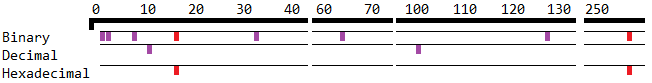
\includegraphics{https://miro.medium.com/max/652/1*1NGffiR_VdV4F7DKSyJ70A.png}

Podemos ver que o binario e o decimal nunca se casam, já o binario e o
hexa sim (eles se casam no 16 e no 255), ou seja, cada 4 bits do binario
( 1000 = 16 0x10) representa um bit no hexadecimal, e esse alinhamento
nos ajuda a representar as coisas, endereços de memoria ..., melhorando
a forma de acessos, paginacao ...

(https://medium.com/@savas/why-do-we-use-hexadecimal-d6d80b56f026 )

    \begin{tcolorbox}[breakable, size=fbox, boxrule=1pt, pad at break*=1mm,colback=cellbackground, colframe=cellborder]
\prompt{In}{incolor}{0}{\hspace{4pt}}
\begin{Verbatim}[commandchars=\\\{\}]
\PY{c+c1}{\PYZsh{} 0000}
\PY{k}{def} \PY{n+nf}{hex2bin}\PY{p}{(}\PY{n}{hex\PYZus{}str}\PY{p}{)}\PY{p}{:}
    \PY{n}{int\PYZus{}} \PY{o}{=} \PY{n+nb}{int}\PY{p}{(}\PY{n}{hex\PYZus{}str}\PY{p}{,}\PY{l+m+mi}{16}\PY{p}{)}
    \PY{n}{bin\PYZus{}str} \PY{o}{=} \PY{l+s+s2}{\PYZdq{}}\PY{l+s+s2}{\PYZdq{}}
    \PY{c+c1}{\PYZsh{} poderiamos usar a funcao a baixo, mas codamos na mao a conversao}
    \PY{c+c1}{\PYZsh{} de hexa \PYZhy{}\PYZgt{} bin \PYZhy{}\PYZhy{}\PYZgt{}\PYZgt{} bin\PYZus{}str2 = str(bin(int\PYZus{}).replace(\PYZdq{}0b\PYZdq{}, \PYZdq{}0\PYZdq{}))}

    \PY{k}{while} \PY{n}{int\PYZus{}} \PY{o}{\PYZgt{}} \PY{l+m+mi}{0}\PY{p}{:} 
        \PY{n}{bin\PYZus{}str} \PY{o}{=} \PY{n+nb}{str}\PY{p}{(}\PY{n}{int\PYZus{}} \PY{o}{\PYZpc{}} \PY{l+m+mi}{2}\PY{p}{)} \PY{o}{+} \PY{n}{bin\PYZus{}str}
        \PY{n}{int\PYZus{}} \PY{o}{=} \PY{n}{int\PYZus{}} \PY{o}{\PYZgt{}\PYZgt{}} \PY{l+m+mi}{1}
    \PY{n}{bin\PYZus{}str} \PY{o}{=}  \PY{l+s+s2}{\PYZdq{}}\PY{l+s+s2}{0}\PY{l+s+s2}{\PYZdq{}}\PY{o}{*}\PY{p}{(}\PY{l+m+mi}{4} \PY{o}{\PYZhy{}} \PY{n+nb}{len}\PY{p}{(}\PY{n}{bin\PYZus{}str}\PY{p}{)}\PY{p}{)} \PY{o}{+} \PY{n}{bin\PYZus{}str}
    \PY{c+c1}{\PYZsh{} por algum motivo ele tira o 0 da frente,}
    \PY{c+c1}{\PYZsh{} segundo um cara na internet isso também acontece com ruby}
    
    \PY{n}{bin\PYZus{}str} \PY{o}{=}  \PY{l+s+s2}{\PYZdq{}}\PY{l+s+s2}{0}\PY{l+s+s2}{\PYZdq{}} \PY{o}{+} \PY{n}{bin\PYZus{}str} 
    
    \PY{k}{return} \PY{n}{bin\PYZus{}str}
\end{Verbatim}
\end{tcolorbox}

    \begin{tcolorbox}[breakable, size=fbox, boxrule=1pt, pad at break*=1mm,colback=cellbackground, colframe=cellborder]
\prompt{In}{incolor}{0}{\hspace{4pt}}
\begin{Verbatim}[commandchars=\\\{\}]
\PY{k}{def} \PY{n+nf}{challenge1}\PY{p}{(}\PY{p}{)}\PY{p}{:}
    \PY{n}{binstr} \PY{o}{=} \PY{n}{hex2bin}\PY{p}{(}\PY{l+s+s2}{\PYZdq{}}\PY{l+s+s2}{49276d206b696c6c696e6720796f757220627261696e206c696b6520}\PY{l+s+se}{\PYZbs{}}
\PY{l+s+s2}{    6120706f69736f6e6f7573206d757368726f6f6d}\PY{l+s+s2}{\PYZdq{}}\PY{p}{)}
    \PY{n}{ret} \PY{o}{=} \PY{n}{b64encode}\PY{p}{(}\PY{n}{binstr}\PY{p}{)}
    \PY{n}{validator}\PY{p}{(}\PY{n}{ret}\PY{p}{)}
    \PY{n+nb}{print}\PY{p}{(}\PY{n}{ret}\PY{p}{)}
    
\PY{n}{challenge1}\PY{p}{(}\PY{p}{)}
    
\end{Verbatim}
\end{tcolorbox}

    \begin{Verbatim}[commandchars=\\\{\}]
FFrom hex to b64 with success!
SSdtIGtpbGxpbmcgeW91ciBicmFpbiBsaWtlIGEgcG9pc29ub3VzIG11c2hyb29t
\end{Verbatim}

    \subsection{Challenge2}\label{challenge2}

https://cryptopals.com/sets/1/challenges/2

Dado duas entradas de mesmo tamanho fazer o xor entre elas

\begin{verbatim}
    str1 = 1c0111001f010100061a024b53535009181c
    str2 = 686974207468652062756c6c277320657965
    output = 746865206b696420646f6e277420706c6179
\end{verbatim}

    \begin{tcolorbox}[breakable, size=fbox, boxrule=1pt, pad at break*=1mm,colback=cellbackground, colframe=cellborder]
\prompt{In}{incolor}{0}{\hspace{4pt}}
\begin{Verbatim}[commandchars=\\\{\}]
\PY{k}{def} \PY{n+nf}{validatorChallenge2}\PY{p}{(}\PY{n}{output}\PY{p}{)}\PY{p}{:}
    \PY{n}{expected} \PY{o}{=} \PY{l+s+s2}{\PYZdq{}}\PY{l+s+s2}{746865206b696420646f6e277420706c6179}\PY{l+s+s2}{\PYZdq{}}
    \PY{k}{if} \PY{n+nb}{str}\PY{p}{(}\PY{n}{output}\PY{p}{)} \PY{o}{==} \PY{n}{expected}\PY{p}{:}
        \PY{n+nb}{print}\PY{p}{(}\PY{l+s+s2}{\PYZdq{}}\PY{l+s+s2}{Funcionou}\PY{l+s+s2}{\PYZdq{}}\PY{p}{)}
        \PY{k}{return} \PY{k+kc}{True}
    \PY{k}{else}\PY{p}{:}
        \PY{n+nb}{print}\PY{p}{(}\PY{l+s+s2}{\PYZdq{}}\PY{l+s+s2}{==ERRO }\PY{l+s+se}{\PYZbs{}n}\PY{l+s+s2}{ sua saída:}\PY{l+s+s2}{\PYZdq{}}\PY{o}{+} \PY{n+nb}{str}\PY{p}{(}\PY{n}{output}\PY{p}{)} \PY{o}{+} \PY{l+s+s2}{\PYZdq{}}\PY{l+s+se}{\PYZbs{}n}\PY{l+s+s2}{ saida esperada:}\PY{l+s+s2}{\PYZdq{}} \PY{o}{+}
              \PY{n+nb}{str}\PY{p}{(}\PY{n}{expected}\PY{p}{)}\PY{p}{)}
        \PY{k}{return} \PY{k+kc}{False}
        
\end{Verbatim}
\end{tcolorbox}

    \paragraph{O que é um XOR?}\label{o-que-uxe9-um-xor}

Xor é uma operação lógica que, dado duas entradas A e B, ela retorna o
valor verdadeiro (1) caso uma entrada tenha o valor diferente da outra.

Tabela verdade da operação :

A \textbar{} B \textbar{} OUTPUT

0 \textbar{} 1 \textbar{} 1

0 \textbar{} 0 \textbar{} 0

1 \textbar{} 1 \textbar{} 0

1 \textbar{} 0 \textbar{} 1

\paragraph{Porque essa operação é tão usada na criptografia
?}\label{porque-essa-operauxe7uxe3o-uxe9-tuxe3o-usada-na-criptografia}

A primeira razão é que Xor é uma função que se aplicada nela mesmo ela
volta pro valor original, ou seja, se tivermos uma string A (string) e
uma chave B, e aplicamos o xor de B em A teremos a string encriptada C.
Como xor é uma função que aplicada a ela mesmo ela retorna pro valor
inicial, ao aplicarmos B xor C teremos A.

A segunda razão é que é uma funcao que não \emph{perde informação}. O
que isso quer dizer, se utilizassemos um 'and' na nossa string A com B,
poderiamos fazer um bruteforce com uma sequencia de 1's, e saberiamos
onde todos os 1s estao, porque na tabela logica do and, só da 1 se ambos
os lados forem 1, com o OR os 0's seriam leakados (bruteforce nos 0s).
Já com o XOR, para termos um output 1 podemos ter como entrada 0 ou 1 e
para ter o output 0 também podemos ter duas entradas possíveis,
dificultando um possível bruteforce.

https://stackoverflow.com/questions/1379952/why-is-xor-used-in-cryptography

    \begin{tcolorbox}[breakable, size=fbox, boxrule=1pt, pad at break*=1mm,colback=cellbackground, colframe=cellborder]
\prompt{In}{incolor}{0}{\hspace{4pt}}
\begin{Verbatim}[commandchars=\\\{\}]
\PY{l+s+sd}{\PYZsq{}\PYZsq{}\PYZsq{}}
\PY{l+s+sd}{essa funcao recebe duas \PYZsq{}strings binarias\PYZsq{} }
\PY{l+s+sd}{\PYZsq{}\PYZsq{}\PYZsq{}}
\PY{k}{def} \PY{n+nf}{xor2xor}\PY{p}{(}\PY{n}{in1}\PY{p}{,}\PY{n}{in2}\PY{p}{)}\PY{p}{:}
    \PY{n}{tam} \PY{o}{=} \PY{n+nb}{len}\PY{p}{(}\PY{n}{in1}\PY{p}{)} \PY{c+c1}{\PYZsh{} tem o mesmo tamanho os dois}
    \PY{n}{ans} \PY{o}{=} \PY{l+s+s2}{\PYZdq{}}\PY{l+s+s2}{\PYZdq{}}
    \PY{k}{for} \PY{n}{i} \PY{o+ow}{in} \PY{n+nb}{range}\PY{p}{(}\PY{l+m+mi}{0}\PY{p}{,} \PY{n+nb}{len}\PY{p}{(}\PY{n}{in1}\PY{p}{)}\PY{p}{)}\PY{p}{:}
        \PY{c+c1}{\PYZsh{} int pra converter de char/string pra int}
        \PY{n}{ans} \PY{o}{+}\PY{o}{=} \PY{n+nb}{str}\PY{p}{(}\PY{n+nb}{int}\PY{p}{(}\PY{n}{in1}\PY{p}{[}\PY{n}{i}\PY{p}{]}\PY{p}{)} \PY{o}{\PYZca{}} \PY{n+nb}{int}\PY{p}{(}\PY{n}{in2}\PY{p}{[}\PY{n}{i}\PY{p}{]}\PY{p}{)}\PY{p}{)}  
    \PY{k}{return} \PY{n}{ans}
\end{Verbatim}
\end{tcolorbox}

    \begin{tcolorbox}[breakable, size=fbox, boxrule=1pt, pad at break*=1mm,colback=cellbackground, colframe=cellborder]
\prompt{In}{incolor}{0}{\hspace{4pt}}
\begin{Verbatim}[commandchars=\\\{\}]
\PY{n}{str1} \PY{o}{=} \PY{l+s+s2}{\PYZdq{}}\PY{l+s+s2}{1c0111001f010100061a024b53535009181c}\PY{l+s+s2}{\PYZdq{}}
\PY{n}{str2} \PY{o}{=} \PY{l+s+s2}{\PYZdq{}}\PY{l+s+s2}{686974207468652062756c6c277320657965}\PY{l+s+s2}{\PYZdq{}}

\PY{k}{def} \PY{n+nf}{challenge2}\PY{p}{(}\PY{p}{)}\PY{p}{:}
    \PY{n}{ans} \PY{o}{=} \PY{l+s+s2}{\PYZdq{}}\PY{l+s+s2}{\PYZdq{}}
    \PY{k}{for} \PY{n}{i} \PY{o+ow}{in} \PY{n+nb}{range}\PY{p}{(}\PY{l+m+mi}{0}\PY{p}{,}\PY{n+nb}{len}\PY{p}{(}\PY{n}{str1}\PY{p}{)}\PY{p}{)}\PY{p}{:}
        \PY{c+c1}{\PYZsh{} }
        \PY{n}{v1} \PY{o}{=} \PY{n}{hex2bin}\PY{p}{(}\PY{n}{str1}\PY{p}{[}\PY{n}{i}\PY{p}{]}\PY{p}{)}
        \PY{n}{v2} \PY{o}{=} \PY{n}{hex2bin}\PY{p}{(}\PY{n}{str2}\PY{p}{[}\PY{n}{i}\PY{p}{]}\PY{p}{)}
        \PY{n}{ans} \PY{o}{+}\PY{o}{=} \PY{n+nb}{hex}\PY{p}{(}\PY{n+nb}{int}\PY{p}{(}\PY{n}{xor2xor}\PY{p}{(}\PY{n}{v1}\PY{p}{,}\PY{n}{v2}\PY{p}{)}\PY{p}{,}\PY{l+m+mi}{2}\PY{p}{)}\PY{p}{)}
    
    \PY{n}{ans} \PY{o}{=} \PY{n}{ans}\PY{o}{.}\PY{n}{replace}\PY{p}{(}\PY{l+s+s1}{\PYZsq{}}\PY{l+s+s1}{0x}\PY{l+s+s1}{\PYZsq{}}\PY{p}{,} \PY{l+s+s1}{\PYZsq{}}\PY{l+s+s1}{\PYZsq{}}\PY{p}{)}
    \PY{n}{validatorChallenge2}\PY{p}{(}\PY{n}{ans}\PY{p}{)}
    \PY{k}{return} \PY{n}{ans}
    
\PY{n+nb}{print}\PY{p}{(}\PY{n}{challenge2}\PY{p}{(}\PY{p}{)}\PY{p}{)}
\PY{c+c1}{\PYZsh{}xored = int(xor2xor(vim,vim2),2)}
\end{Verbatim}
\end{tcolorbox}

    \begin{Verbatim}[commandchars=\\\{\}]
Funcionou
746865206b696420646f6e277420706c6179
\end{Verbatim}

    \subsection{challenge 5}\label{challenge-5}

Para última challenge da TAG foi feita a challenge 5 (
https://cryptopals.com/sets/1/challenges/5 ) Basicamente ela faz uso dos
últimos códigos e consiste em pegar uma string :

\begin{verbatim}
        Burning 'em, if you ain't quick and nimble
        I go crazy when I hear a cymbal
\end{verbatim}

e aplicar uma chave pra encriptarmos ela com o xor. no caso a chave é
\emph{ICE}.

Como a chave é menos que a string completa, vamos aplicando ICE até o
final repetidamente.

\begin{verbatim}
ICEICEICEICEIC...
letra por letra.
\end{verbatim}

    \begin{tcolorbox}[breakable, size=fbox, boxrule=1pt, pad at break*=1mm,colback=cellbackground, colframe=cellborder]
\prompt{In}{incolor}{0}{\hspace{4pt}}
\begin{Verbatim}[commandchars=\\\{\}]
\PY{n}{str1} \PY{o}{=} \PY{n}{b}\PY{l+s+s2}{\PYZdq{}}\PY{l+s+s2}{Burning }\PY{l+s+s2}{\PYZsq{}}\PY{l+s+s2}{em, if you ain}\PY{l+s+s2}{\PYZsq{}}\PY{l+s+s2}{t quick and nimble}\PY{l+s+se}{\PYZbs{}n}\PY{l+s+s2}{I go crazy when I hear}\PY{l+s+se}{\PYZbs{}}
\PY{l+s+s2}{ a cymbal}\PY{l+s+s2}{\PYZdq{}}
\PY{n}{key}  \PY{o}{=} \PY{n}{b}\PY{l+s+s2}{\PYZdq{}}\PY{l+s+s2}{ICE}\PY{l+s+s2}{\PYZdq{}}

\PY{c+c1}{\PYZsh{} zerofill deixa os dois bytes, o da chave e o da string do mesmo tamanho .}
\PY{c+c1}{\PYZsh{} ele coloca zeros na frente até terem o mesmo tamanho}
\PY{k}{def} \PY{n+nf}{zerofill}\PY{p}{(}\PY{n}{st}\PY{p}{,}\PY{n}{l}\PY{p}{)}\PY{p}{:}
    \PY{k}{return} \PY{l+s+s1}{\PYZsq{}}\PY{l+s+s1}{0}\PY{l+s+s1}{\PYZsq{}}\PY{o}{*}\PY{p}{(}\PY{n}{l} \PY{o}{\PYZhy{}} \PY{n+nb}{len}\PY{p}{(}\PY{n}{st}\PY{p}{)}\PY{p}{)} \PY{o}{+} \PY{n}{st}

\PY{c+c1}{\PYZsh{} esse xor2xor2 eh a mesma coisa que o xor2xor, eu so mudei ele porque estava }
\PY{c+c1}{\PYZsh{} tendo problemas e achei que poderia ser ele}
\PY{c+c1}{\PYZsh{} e,claro, ele usa list comprehension}
\PY{c+c1}{\PYZsh{} como gostei da solucao com listcomprehension resolvei deixar}
\PY{k}{def} \PY{n+nf}{xor2xor2}\PY{p}{(}\PY{n}{in1}\PY{p}{,}\PY{n}{in2}\PY{p}{)}\PY{p}{:}
    \PY{l+s+sd}{\PYZsq{}\PYZsq{}\PYZsq{}}
\PY{l+s+sd}{    tam = len(in1) \PYZsh{} tem o mesmo tamanho os dois}
\PY{l+s+sd}{    ans = \PYZdq{}\PYZdq{}}
\PY{l+s+sd}{    for i in range(0, len(in1)):}
\PY{l+s+sd}{        ans += str(int(in1[i]) \PYZca{} int(in2[i])) }
\PY{l+s+sd}{    \PYZsq{}\PYZsq{}\PYZsq{}}
    \PY{k}{return} \PY{p}{(}\PY{p}{[}\PY{n+nb}{int}\PY{p}{(}\PY{n}{in1}\PY{p}{[}\PY{n}{i}\PY{p}{]}\PY{p}{)} \PY{o}{\PYZca{}} \PY{n+nb}{int}\PY{p}{(}\PY{n}{in2}\PY{p}{[}\PY{n}{i}\PY{p}{]}\PY{p}{)} \PY{k}{for} \PY{n}{i} \PY{o+ow}{in} \PY{n+nb}{range}\PY{p}{(}\PY{n+nb}{len}\PY{p}{(}\PY{n}{in1}\PY{p}{)}\PY{p}{)}\PY{p}{]}\PY{p}{)}
\PY{k}{def} \PY{n+nf}{ch5}\PY{p}{(}\PY{n}{s}\PY{p}{,}\PY{n}{key}\PY{p}{)}\PY{p}{:}
    \PY{n}{i\PYZus{}key} \PY{o}{=} \PY{l+m+mi}{0} \PY{c+c1}{\PYZsh{} index of key, max = 2... 0,1,2}
    \PY{n}{keyBin} \PY{o}{=} \PY{p}{[}\PY{p}{]}

    \PY{k}{for} \PY{n}{byte} \PY{o+ow}{in} \PY{n}{key} \PY{p}{:}
        \PY{n}{keyBin}\PY{o}{.}\PY{n}{append}\PY{p}{(}\PY{n+nb}{format}\PY{p}{(}\PY{n}{byte}\PY{p}{,}\PY{l+s+s1}{\PYZsq{}}\PY{l+s+s1}{b}\PY{l+s+s1}{\PYZsq{}}\PY{p}{)}\PY{p}{)}

    \PY{n}{ans} \PY{o}{=}  \PY{l+s+s1}{\PYZsq{}}\PY{l+s+s1}{\PYZsq{}}
    \PY{k}{for} \PY{n}{byte} \PY{o+ow}{in} \PY{n}{s}\PY{p}{:}
        \PY{n}{bs} \PY{o}{=} \PY{n+nb}{format}\PY{p}{(}\PY{n}{byte}\PY{p}{,}\PY{l+s+s1}{\PYZsq{}}\PY{l+s+s1}{b}\PY{l+s+s1}{\PYZsq{}}\PY{p}{)}
        \PY{k}{if} \PY{n+nb}{len}\PY{p}{(}\PY{n}{bs}\PY{p}{)} \PY{o}{\PYZlt{}} \PY{n+nb}{len}\PY{p}{(}\PY{n}{keyBin}\PY{p}{[}\PY{n}{i\PYZus{}key}\PY{p}{]}\PY{p}{)}\PY{p}{:}
            \PY{n}{bs} \PY{o}{=} \PY{n}{zerofill}\PY{p}{(}\PY{n}{bs}\PY{p}{,}\PY{n+nb}{len}\PY{p}{(}\PY{n}{keyBin}\PY{p}{[}\PY{n}{i\PYZus{}key}\PY{p}{]}\PY{p}{)}\PY{p}{)}
            
        \PY{n}{xx2} \PY{o}{=} \PY{n}{xor2xor2}\PY{p}{(}\PY{n}{bs}\PY{p}{,}\PY{n}{keyBin}\PY{p}{[}\PY{n}{i\PYZus{}key}\PY{p}{]}\PY{p}{)}
        \PY{n}{bits\PYZus{}string}\PY{o}{=}  \PY{l+s+s1}{\PYZsq{}}\PY{l+s+s1}{\PYZsq{}}\PY{o}{.}\PY{n}{join}\PY{p}{(}\PY{n+nb}{map}\PY{p}{(}\PY{n+nb}{str}\PY{p}{,} \PY{n}{xx2}\PY{p}{)}\PY{p}{)}
        
        \PY{c+c1}{\PYZsh{} esse if so funciona no caso desse exercicio}
        \PY{c+c1}{\PYZsh{} por alguma razao, como boa parte das coisas tentei fazer handmade,}
        \PY{c+c1}{\PYZsh{} por alguma razao ao trabalhar com os bits}
        \PY{c+c1}{\PYZsh{} o python ao inves de colocar 0x0b 0x0a e 0x0c, ele coloca apenas}
        \PY{c+c1}{\PYZsh{} 0xa 0xb 0xc. }
        \PY{c+c1}{\PYZsh{} e esses bits que ele comeu fizeram falta na  resposta final. }
        \PY{c+c1}{\PYZsh{} O codigo abaixo foi um remendo pra isso ai.}

        \PY{n}{value} \PY{o}{=} \PY{n+nb}{hex}\PY{p}{(}\PY{n+nb}{int}\PY{p}{(}\PY{n}{bits\PYZus{}string}\PY{p}{,}\PY{l+m+mi}{2}\PY{p}{)}\PY{p}{)}
        \PY{n}{carelist} \PY{o}{=} \PY{p}{[}\PY{l+s+s1}{\PYZsq{}}\PY{l+s+s1}{0xa}\PY{l+s+s1}{\PYZsq{}}\PY{p}{,}\PY{l+s+s1}{\PYZsq{}}\PY{l+s+s1}{0xb}\PY{l+s+s1}{\PYZsq{}}\PY{p}{,}\PY{l+s+s1}{\PYZsq{}}\PY{l+s+s1}{0xc}\PY{l+s+s1}{\PYZsq{}}\PY{p}{,}\PY{l+s+s1}{\PYZsq{}}\PY{l+s+s1}{0xd}\PY{l+s+s1}{\PYZsq{}}\PY{p}{,}\PY{l+s+s1}{\PYZsq{}}\PY{l+s+s1}{0xe}\PY{l+s+s1}{\PYZsq{}}\PY{p}{,}\PY{l+s+s1}{\PYZsq{}}\PY{l+s+s1}{0xf}\PY{l+s+s1}{\PYZsq{}}\PY{p}{]}
        \PY{k}{if} \PY{n}{value} \PY{o+ow}{in} \PY{n}{carelist}\PY{p}{:}
            \PY{n}{tmp} \PY{o}{=} \PY{n}{value}\PY{o}{.}\PY{n}{replace}\PY{p}{(}\PY{l+s+s1}{\PYZsq{}}\PY{l+s+s1}{0x}\PY{l+s+s1}{\PYZsq{}}\PY{p}{,} \PY{l+s+s1}{\PYZsq{}}\PY{l+s+s1}{\PYZsq{}}\PY{p}{)}
            \PY{n}{value} \PY{o}{=} \PY{l+s+s1}{\PYZsq{}}\PY{l+s+s1}{0x0}\PY{l+s+s1}{\PYZsq{}} \PY{o}{+} \PY{n}{tmp}
            
        \PY{n}{ans} \PY{o}{+}\PY{o}{=} \PY{n}{value}
        \PY{c+c1}{\PYZsh{} seta o index da key}
        \PY{k}{if} \PY{p}{(}\PY{n}{i\PYZus{}key} \PY{p}{)} \PY{o}{==} \PY{l+m+mi}{2} \PY{p}{:}
            \PY{n}{i\PYZus{}key} \PY{o}{=} \PY{l+m+mi}{0}
        \PY{k}{else} \PY{p}{:}
            \PY{n}{i\PYZus{}key} \PY{o}{+}\PY{o}{=} \PY{l+m+mi}{1} 
    \PY{k}{return} \PY{n}{ans}

\PY{n}{v} \PY{o}{=} \PY{n}{ch5}\PY{p}{(}\PY{n}{str1}\PY{p}{,}\PY{n}{key}\PY{p}{)}\PY{o}{.}\PY{n}{replace}\PY{p}{(}\PY{l+s+s1}{\PYZsq{}}\PY{l+s+s1}{0x}\PY{l+s+s1}{\PYZsq{}}\PY{p}{,} \PY{l+s+s1}{\PYZsq{}}\PY{l+s+s1}{\PYZsq{}}\PY{p}{)}
\PY{n+nb}{print}\PY{p}{(}\PY{n}{v}\PY{p}{)}

\PY{n}{expected} \PY{o}{=} \PY{l+s+s2}{\PYZdq{}}\PY{l+s+s2}{0b3637272a2b2e63622c2e69692a23693a2a3c6324202d623d63343c2a26226324}\PY{l+s+se}{\PYZbs{}}
\PY{l+s+s2}{272765272a282b2f20430a652e2c652a3124333a653e2b2027630c692b20283165286326302e27}\PY{l+s+se}{\PYZbs{}}
\PY{l+s+s2}{282f}\PY{l+s+s2}{\PYZdq{}}
\PY{k}{assert}\PY{p}{(}\PY{n}{v} \PY{o}{==} \PY{n}{expected}\PY{p}{)}

\PY{c+c1}{\PYZsh{} A minha resposta tinha 3 bits de diferença da original, e eu passei boas 3}
\PY{c+c1}{\PYZsh{} horas tentando entender o porque}
\PY{c+c1}{\PYZsh{} basicamente, como eu fiz tudo handmade \PYZhy{} ou quase tudo\PYZhy{} o python ao inves de}
\PY{c+c1}{\PYZsh{} colocar  e 0x0b 0x0a e 0x0c, ele coloca apenas 0xa 0xb 0xc, e os 3 zeros que }
\PY{c+c1}{\PYZsh{} ele \PYZsq{}come\PYZsq{} são os que estavam faltando. Por isso fiz a solucao (gambiarra) do }
\PY{c+c1}{\PYZsh{} carelist}
\end{Verbatim}
\end{tcolorbox}

    \begin{Verbatim}[commandchars=\\\{\}]
0b3637272a2b2e63622c2e69692a23693a2a3c6324202d623d63343c2a26226324272765272a282b
2f20430a652e2c652a3124333a653e2b2027630c692b20283165286326302e27282f
\end{Verbatim}

    \begin{tcolorbox}[breakable, size=fbox, boxrule=1pt, pad at break*=1mm,colback=cellbackground, colframe=cellborder]
\prompt{In}{incolor}{0}{\hspace{4pt}}
\begin{Verbatim}[commandchars=\\\{\}]

\end{Verbatim}
\end{tcolorbox}


    % Add a bibliography block to the postdoc
    
    
    
    \end{document}
